\documentclass[a4paper, 10pt]{article}%тип документа
\usepackage[T2A]{fontenc} %кодировка
\usepackage[utf8]{inputenc} %кодировка исходного кода
\usepackage[english,russian]{babel} %локализация и переносы
\usepackage{multirow}
\usepackage{wrapfig}
\usepackage{graphicx}
\usepackage{mathtext}
\usepackage{amsmath}
\usepackage{siunitx} % Required for alignment
\usepackage{multirow}
\usepackage{rotating}
\usepackage{float}
\usepackage[T1,T2A]{fontenc}
\usepackage[russian]{babel}
\graphicspath{{pictures/}}
%Производные
\usepackage{physics}
%Математика
\usepackage{amsmath, amsfonts, amssymb, amsthm, mathtools}
\usepackage[left=10mm, top=20mm, right=18mm, bottom=15mm, footskip=10mm]{geometry}
\title{1.1.8 Измерение ускорения свободного падения}
\author{Мыздриков Иван, Б06-401}
\date{23 октября 2024 г.}

\begin{document}

\maketitle

\section{Аннотация}
Цель работы: определить ускорение свободного падения посредством прямых измерений ускорения падающего тела. 

В работе используются: вертикальная труба с намотанными катушками; шарообразные неодимовые магниты; линейка; блок регистрации сигнала (микроконтроллер с АЦП), соединённый с цифровым осциллографом. 

\section{Теоретические сведения}
В данной лабораторной работе ускорение свободного падения g определяется при помощи измерения времени падения металлического шарика в поле тяжести Земли. Экспериментальная установка приведена на рис.1. Металлический шарик (неодимовый магнит) первоначально удерживается сверху электромагнитом в подвешенном состоянии. После выключения тока, текущего через электромагнит, шарик начинает падать вниз и пролетает последовательно через шесть тонких проволочных катушек. С катушками соединены датчики электрического напряжения и регистраторы времени (таймеры). Шарик имеет собственную намагниченность (является постоянным магнитом), поэтому, когда он пролетает сквозь проволочную катушку, он своим магнитным полем наводит в катушке индукционный ток. Этот ток регистрируется электрическим датчиком, соединённым с катушкой. По возникающему импульсу напряжения срабатывает таймер, соединённый с данной катушкой.  
Все датчики подключены к блоку управления и регистрации. Начало отсчёта времени t = 0 соответствует пролёту шариком самой верхней катушки. Каждый из таймеров регистрирует время пролёта шариком соответствующей катушки. Расстояние между соседними катушками одинаково и равно l $\approx$ 40 см (точные значения указаны на установке или могут быть измерены непосредственно). На таком же расстоянии находится шарик в подвешенном состоянии над верхней катушкой.  
\begin{figure}[h]
    \centering
    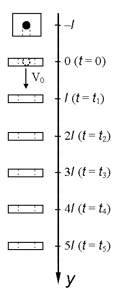
\includegraphics[width=0.15\textwidth]{изображение.png}
    \caption{Схема экспериментальной установки}
    \label{fig:mesh1}
\end{figure}
После пролёта всех катушек шарик попадает в металлическую трубку, в которой он тормозится перед падением на пол (электромагнитное торможение). Механизм торможения заключается в том, что так же, как и в катушках, в металлической трубке наводятся индукционные токи (токи 
Фуко), которые, в соответствии с правилом Рис. 1. Схема опыта Ленца, своим магнитным полем тормозят движение шарика. Заметим, что шарик будет неизбежно испытывать некоторое торможение и при пролёте каждой катушки. Однако этот эффект можно свести к минимуму, если сопротивление цепи катушки достаточно велико, и, следовательно, возникающие токи, а значит и силы, малы.
Импульсы тока от всех катушек также регистрируются на экране запоминающего осциллографа. По картине импульсов на экране осциллографа можно примерно определить время пролёта шариком каждой из катушек и сравнить это время с соответствующим значением таймера. Согласно закону электромагнитной индукции $\epsilon = - \frac{d\Phi}{dt}$ напряжение в цепи регистрации пропорционально производной магнитного потока от шарика через регистрирующую катушку. Поэтому, когда шарик будет находится в центре регистрирующей катушки, поток магнитного поля через неё будет максимален, что будет соответствовать нулю регистрируемого сигнала. Характерный вид осциллограммы представлен на рис. 2. Конкретные амплитуды и форма отдельных импульсов могут меняться как для разных катушек, так и от опыта к опыту: они зависят от ориентации намагниченности шарика относительно катушки в момент пролёта (импульсы с большой амплитудой соответствуют случаю, когда намагниченность шарика направлена вертикально). Рассмотрим падение шарика из его начального положения, когда он удерживается электромагнитом. Направим ось у вертикально вниз, а начало отсчёта y = 0 совместим с положением самой верхней катушки (рис. 1). 
Пусть $V_0$ – скорость шарика в центре самой верхней катушки. Для равноускоренного движения шарика справедливо выражение: 

\[y = V_o t + \frac{g t^2}{2}\]
Это выражение можно записать для пяти моментов времени $t_n$ (n = 1, 2, 3, 4, 5), соответствующих пролёту шарика через соответствующую катушку: 

\[\frac{nl}{t_n} = V_0 + \frac{g t_n}{2}\]
Проводя измерения времён $t_n$ при свободном падении шарика и используя выражение выше, можно построить график зависимости величины $nl/t_n$ от $t_n$  и определить ускорение свободного падения из углового коэффициента данной зависимости. 
\begin{figure}[h]
    \centering
    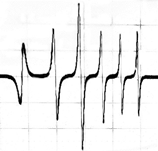
\includegraphics[width=0.15\linewidth]{изображение1.png}
    \caption{Характерная осциллограмма в эксперименте}
    \label{fig:enter-label}
\end{figure}


Влияние сопротивления воздуха* 



Падение шарика в атмосфере не является полностью свободным: он, конечно, испытывает влияние сопротивления воздуха. Из-за этого измеряемое на опыте ускорение g окажется несколько меньше. Точный учёт силы сопротивления потребовал бы либо отдельного экспериментального исследования, либо решения сложной гидродинамической задачи в зависимости от скорости движения $V$. Однако оценить силу сопротивления по порядку величины можно в следующих двух упрощённых моделях. 
При падении с малыми скоростями можно применить известную формулу Стокса*: 

\[F_{\text{сопр}} = 6 \pi \eta r v\]
где $r$ — радиус шара, $\eta$ — вязкость воздуха (при нормальном давлении и комнатной температуре $\eta \approx 1.85 \cdot 10^{-5}$ Па $\cdot $ с). 
При больших скоростях обтекание шарика становится турбулентным и теория Стокса неприменима. Сила оказывается пропорциональна квадрату скорости и площади поперечного сечения шарика: 

\[F_{\text{сопр}} = C \pi r^2 \rho v^2\]
где $\rho$ — плотность воздуха ($\rho \approx 1,2 \text{кг/м}^3$ ), C — константа, зависящая от формы тела, которая для может быть установлена только экспериментально. Для шара известно экспериментальное значение $C_\text{ш}$ $\approx$ 0,2. Заметим, что  эта формула имеет прозрачный физический смысл: величина $\pi r^2 \rho v^2$— это количество импульса, которое сообщали бы в секунду молекулы воздуха шарику при неупругом ударе о него (убедитесь в том самостоятельно). 
Критерием выбора между двумя моделями служит так называемое число 
Рейнольдса:

\[\text{Re} = \frac{\rho v r}{\eta}\]
По своему смыслу число Рейнольдса является отношением кинетической энергии течения жидкости (или газа) к работе сил трения. Формула Cтокса (4) применима, когда влияние трения велико, а число Рейнольдса, соответственно, мало: Re $\leq$ 1. Формула (5) будет, напротив, справедлива при достаточно больших числах Re $\gg$ 1 (на практике при Re > 50). 
В нашей работе высота падения составляет H $\approx$ 2 м, что даёт максимальную скорость падения $v_{max} \approx \sqrt{2gH} \approx 6.3 \text{м/с}$  (сила сопротивления в нашем опыте в любом случае мала, поэтому для грубой оценки скорости падения ей можно пренебречь). При радиусе шарика r $\approx$ 1 см, получим $Re_{max}$ $\sim$ 4 $\cdot$ 103 $\gg$ 1. Следовательно, следует ожидать, что обтекание шарика воздухом в нашем опыте будет заведомо турбулентным почти с самого начала падения, а сила лобового сопротивления пропорциональна квадрату скорости согласно (5). 
Оценить влияние сопротивления воздуха на измеряемое в опыте ускорение вертикального падения можно, вычислив среднюю величину силы (5) и соответствующее ей ускорение: $\Delta g \approx \frac{F_\text{сопр}}{m}$, где m — масса шарика.


\section{Методика измерений}

В данной работе исследуется движение магнита вниз по вертикальной трубе. Регистрация положения магнита в зависимости от времени осуществляется электромагнитными датчиками. Для этого на внешнюю поверхность трубы намотана система катушек. Все катушки соединены последовательно (намотаны из одного провода). Прохождение магнита через каждую катушку приводит, ввиду явления электромагнитной индукции, к генерации импульса напряжения во всей цепи. 

%\begin{figure}[h]
 %   \centering
  %  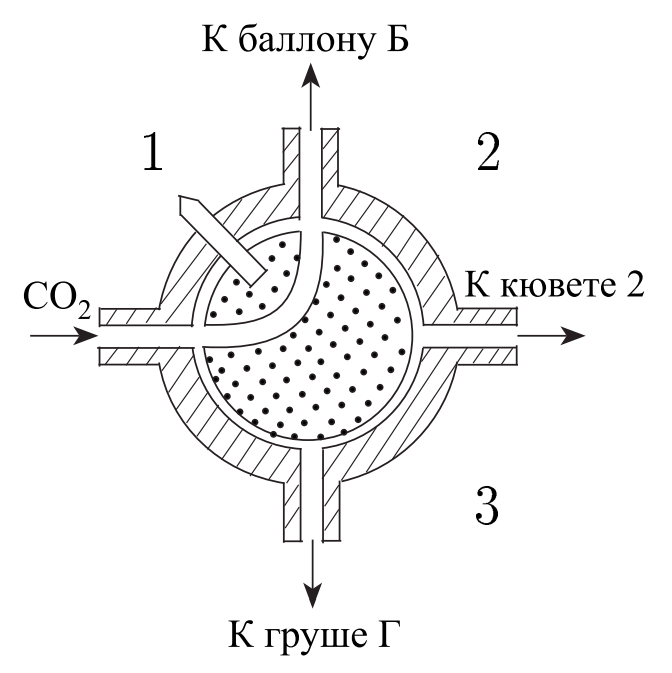
\includegraphics[width=0.4\linewidth]{pic3.jpeg}
   % \caption{Экспериментальная установка}
    %\label{fig:enter-label}
%\end{%figure}

\paragraph{Действия, которые небоходимо сделать в ходе работы:}
\begin{enumerate}
    \item Первым делом необходимо ознакомиться с экспериментальной установкой и убедиться, что расстояние между катушками одинаково.
    \item Подготовьте все приборы к работе (включите их, у электромагнита должен загореться красный световой индикатор)
    \item Проведите измерения необходимых для расчетов параметров магнита - радиуса и массы. Важно отметить, что шарик - очень сильный магнит. Необходимо не допускать его сближения с металлическими поверхностями и другими магнитами. 
    \item Положите шарик в пластиковый держатель, закреплённый на длинной ме-
таллической штанге, и поднесите его к установленному в верхней точке
установки электромагниту так, чтобы он зафиксировался в нём.
\item При нажатии кнопки «Сброс» на блоке управления произойдёт размыкание
электрической цепи электромагнита, и шарик свободно упадёт вниз.
Наблюдайте на экране осциллографа осциллограмму сигнала от пролёта
шарика.
\item С помощью осциллографа измерьте времена пролёта
магнита через катушки. Проведите измерения 7-10 раз. 
Сравните результаты со значениями,
отображаемыми на цифровом индикаторе блока регистрации.
\item По полученным данным постройте графики зависимости. Оцените погрешность результата

\end{enumerate}

\section{Используемое оборудование}
Оценка погрешности измерений:

После длительных вычислений получим, что силой сопротивления воздуха можно пренебречь. Инструментальная погрешность длины между соседними катушками составляет 1мм.Остальные погрешности можно оценить только во время практической работы

Перечень измерительных приборов, используемых в работе:
\begin{enumerate}
    \item Линейка $\pm 0.1$ см
    \item Блок регистрации сигнала
    \item Цифровой осциллограф
\end{enumerate}

\section{Результаты измерений и обработка данных}

Полученные данные:

l=37.5см

Занесём результаты 1 броска в таблицу 1
\begin{table}[!ht]
    \centering
    \begin{tabular}{|l|l|l|l|l|l|}
    \hline
        l,м & 0.375 & 0.75 & 1.125 & 1.5 & 1.875 \\ \hline
        t,с & 0.12 & 0.207 & 0.284 & 0.351 & 0.412 \\ \hline
    \end{tabular}
    \caption{1 бросок}
\end{table}

\newpage
Занесём результаты 2 броска в таблицу 2
\begin{table}[!ht]
    \centering
    \begin{tabular}{|l|l|l|l|l|l|}
    \hline
        l,м & 0.375 & 0.75 & 1.125 & 1.5 & 1.875 \\ \hline
        t,с & 0.118 & 0.207 & 0.283 & 0.35 & 0.41 \\ \hline
    \end{tabular}
    \caption{2 бросок}
\end{table}

Занесём результаты 3 броска в таблицу 3
\begin{table}[!ht]
    \centering
    \begin{tabular}{|l|l|l|l|l|l|}
    \hline
        l,м & 0.375 & 0.75 & 1.125 & 1.5 & 1.875 \\ \hline
        t,с & 0.119 & 0.207 & 0.283 & 0.350 & 0.41 \\ \hline
    \end{tabular}
    \caption{3 бросок}
\end{table}

Занесём результаты 4 броска в таблицу 4
\begin{table}[!ht]
    \centering
    \begin{tabular}{|l|l|l|l|l|l|}
    \hline
        l,м & 0.375 & 0.75 & 1.125 & 1.5 & 1.875 \\ \hline
        t,с & 0.12 & 0.207 & 0.283 & 0.350 & 0.411 \\ \hline
    \end{tabular}
    \caption{4 бросок}
\end{table}

По полученным данным построим графики зависимости  от  и по
угловому коэффициенту наилучшей прямой определите ускорение свободного падения

График 1
\begin{figure}[h!]
    \centering
    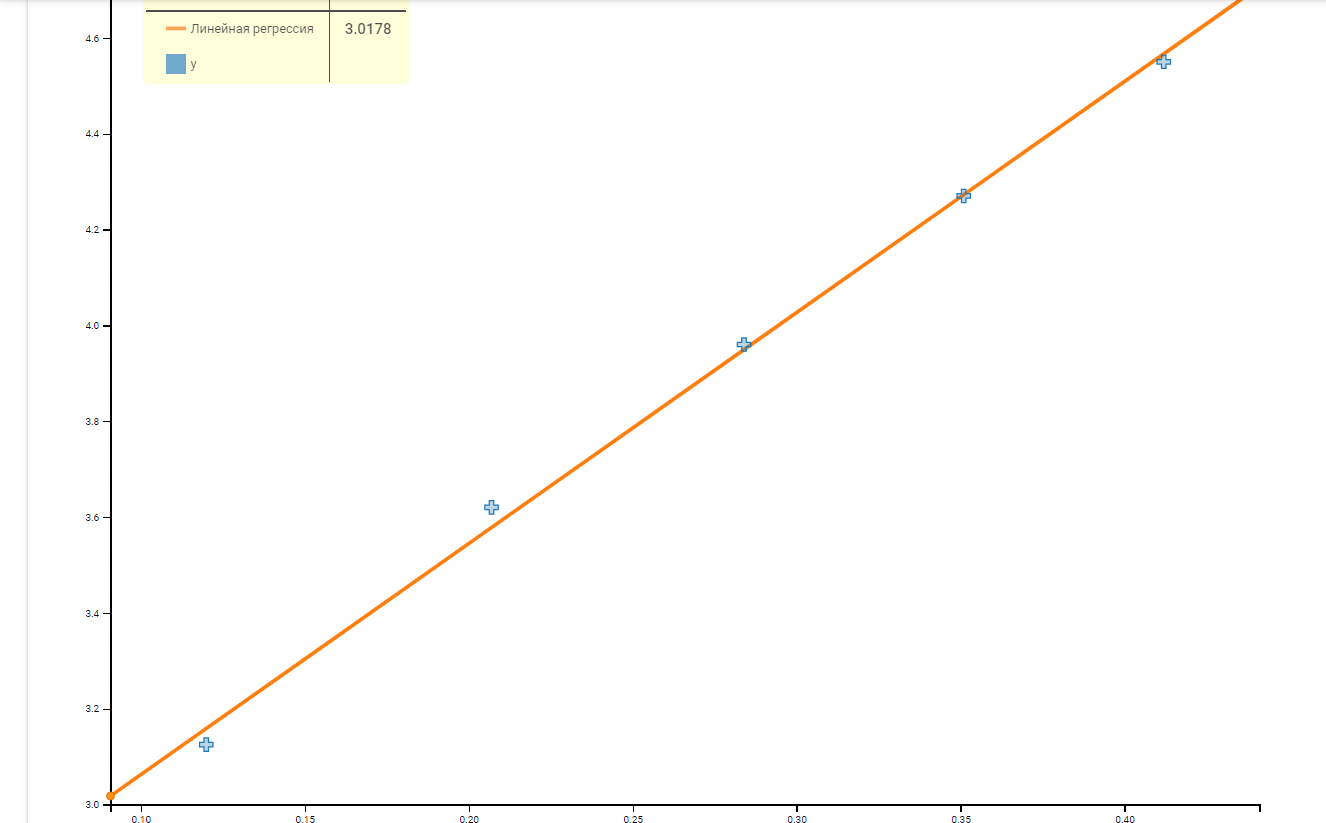
\includegraphics[width=0.15\linewidth]{график 1.png}
    \caption{Зависимость nl/t_{n} \hspace{3pt} \text{от} \hspace{3pt}t_{n}}
    \label{fig:enter-label}
\end{figure}

График 2
\begin{figure}[h!]
    \centering
    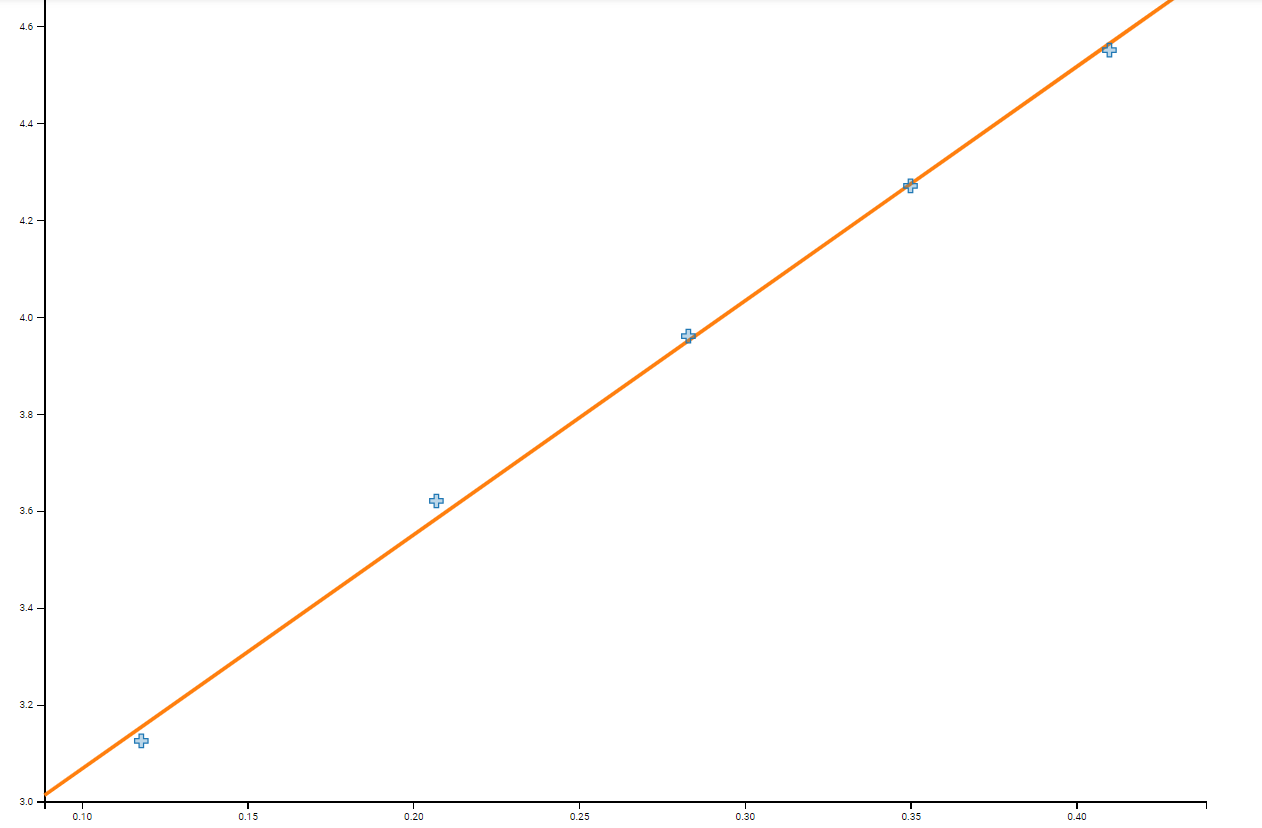
\includegraphics[width=0.15\linewidth]{график 2.png}
    \caption{Зависимость nl/t_{n} \hspace{3pt} \text{от} \hspace{3pt}t_{n}}
    \label{fig:enter-label}
\end{figure}

График 3
\begin{figure}[h!]
    \centering
    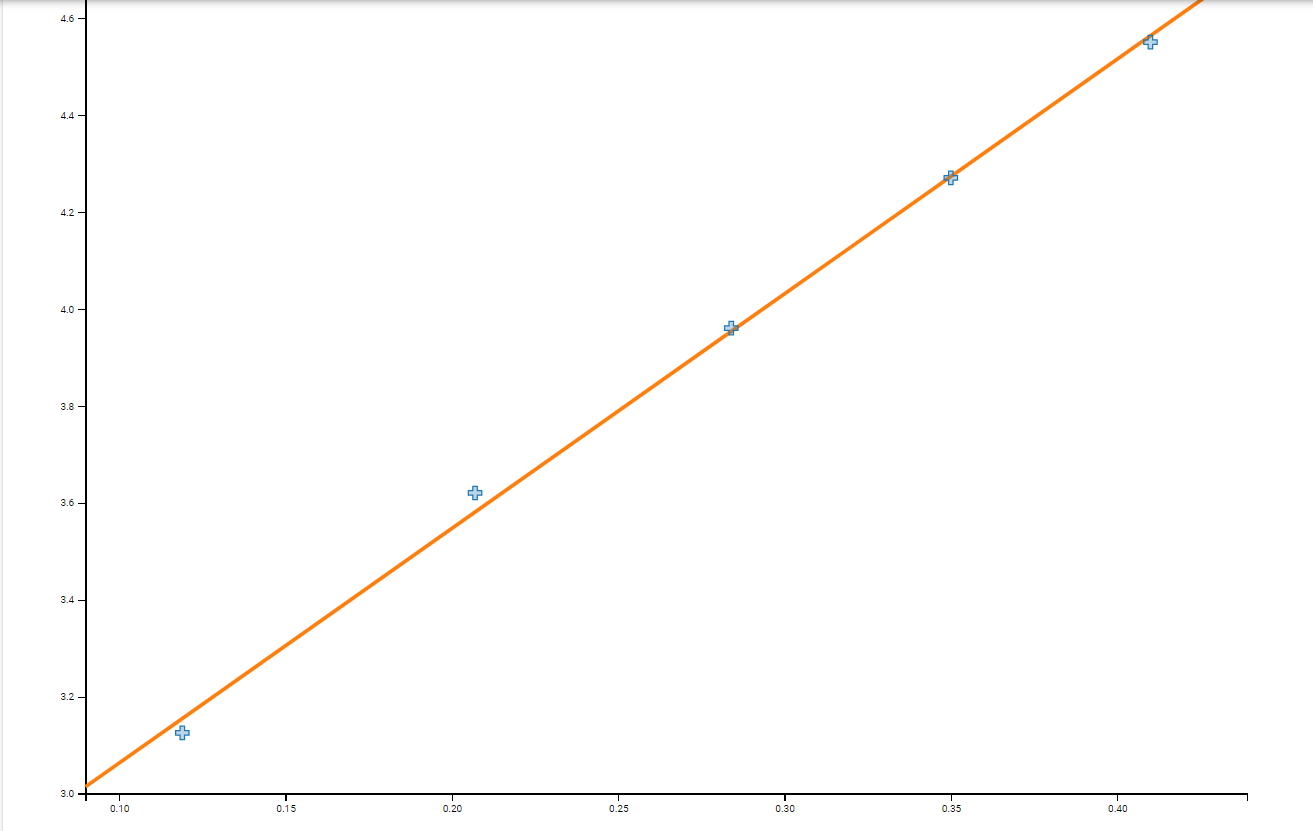
\includegraphics[width=0.15\linewidth]{график 3.png}
    \caption{Зависимость nl/t_{n} \hspace{3pt} \text{от} \hspace{3pt}t_{n}}
    \label{fig:enter-label}
\end{figure}

График 4
\begin{figure}[h!]
    \centering
    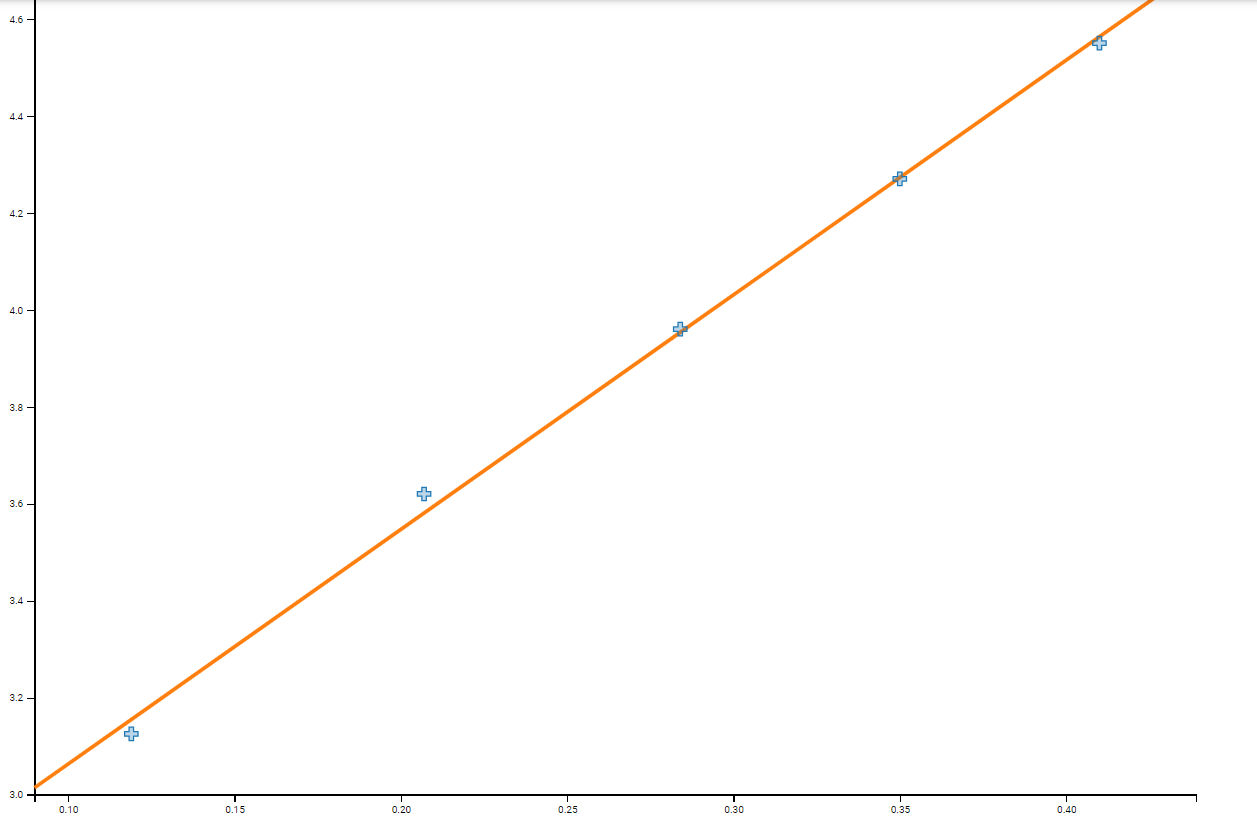
\includegraphics[width=0.15\linewidth]{график 4.png}
    \caption{Зависимость nl/t_{n} \hspace{3pt} \text{от} \hspace{3pt}t_{n}}
    \label{fig:enter-label}
\end{figure}

Исходя из первого графика g$\approx$ 9.74 $\frac{\text{м}}{\text{с}^2}$

Исходя из второго графика g$\approx$ 9.73 $\frac{\text{м}}{\text{с}^2}$

Исходя из третьего графика g$\approx$ 9.74 $\frac{\text{м}}{\text{с}^2}$

Исходя из четвёртого графика g$\approx$ 9.74 $\frac{\text{м}}{\text{с}^2}$

Таким образом $\text{g}_\text{ср} \approx$ 9.737 $\frac{\text{м}}{\text{с}^2}$

\section{Обсуждение результатов}
В ходе работы мы экспериментально получили значение ускорения свободного падения и оценили погрешность.Полученные резульаты укладываются в табличные значения.При помощи 4 бросков мы усреднили значение ускорения свободного падения и учли погрешность различных приборов для измерения величин.

\section{Вывод}
В ходе работы мы получили Зависимость $nl/t_{n}$ \hspace{3pt} от \hspace{3pt}$t_{n}$ и по угловому коэффициенту наилучшей прямой определили ускорение свободного падения, равное $\text{g}_\text{ср} \approx$ 9.737$\frac{\text{м}}{\text{с}^2}$. Итоговая погрешность составила $\pm 0.17 \frac{\text{м}}{\text{с}^2}$




\end{document}
